% !TEX encoding = UTF-8
% !TEX program = xelatex
\documentclass[12pt,a4paper]{article}
\usepackage[paperwidth=210mm, paperheight=297mm, left=0.75in, right=0.75in, bottom=1in, top=1in]{geometry}
\usepackage{polyglossia}
\setdefaultlanguage[babelshorthands]{italian}
\usepackage{fontspec}
\usepackage{graphicx}
\usepackage{blindtext}
\usepackage{wrapfig}

\frenchspacing
\makeindex

\begin{document}
\title{\vspace{-70pt}IRAS}
\author{Elvis Ruci}
\date{}
\maketitle
\pagestyle{empty}
\thispagestyle{empty}

\section*{Storia}
\label{storia}
\begin{wrapfigure}{r}{0.35\textwidth}
  \vspace{-10pt}
  \begin{center}
    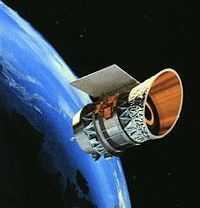
\includegraphics[width=0.30\textwidth]{satellite}
  \end{center}
  \vspace{-20pt}
  %\caption{A gull}
\end{wrapfigure}
Il telescopio spaziale IRAS (Infra Red Astronomical Satellite) fu realizzato dalla collaborazione delle agenzie spaziali di USA, Inghilterra e Olanda.

Lanciato dalla base militare americana di Vandenberg il \emph{25 gennaio 1983}, l'IRAS era per l'epoca il più potente strumento osservativo del cielo ad infrarossi costruito dall'uomo. 

La missione durò meno del previsto (10 mesi) a causa di un guasto che fece evaporare più velocemente del previsto la riserva di elio superfluido usato dal sistema di raffreddamento. 

\section*{Osservazioni}
\label{osservazioni}

Con la celebre forma a cilindro di una tonnellata di peso e 3,25 metri di altezza, racchiudeva un sofisticato sistema di raffreddamento che doveva mantenere il telescopio a specchio di 60 cm, ad una temperatura di 1,6 kelvin (circa −272 °C). Il compito dello strumento era di mappare il cielo alle lunghezze d'onda di 12, 25, 60 e 100 micrometri.

Nonostante la breve durata, \emph{riusci effettivamente a mappare per quattro volte il 96\% della volta celeste} scoprendo circa 500.000 sorgenti infrarosse, di cui circa 75.000 erano galassie starburst, ancora nella loro fase di formazione stellare. Tra i risultati accertati, la scoperta di un anello di polvere cosmica che circonda il Sistema Solare a una distanza di circa 15 miliardi di chilometri e frammenti rocciosi attorno a Vega, ritenuto dagli astronomi un sistema planetario in formazione.

Jack Meadows e colleghi utilizzarono i risultati per scoprire tre asteroidi (tra cui 3200 Phaethon e un asteroide Apollo), sei comete e una grande coda di polveri associata alla cometa Tempel--2.

\section*{Curiosità}
\label{curiosit}

Il telescopio IRAS oltre che mappare il cielo agli infrarossi, probabilmente fu mandato nello spazio anche per verificare la presenza di eventuali corpi transplutoniani super freddi ai confini del Sistema Solare. L'idea che potesse esistere il \emph{``Tenth Planet''}, a quei tempi era molto probabile.

Si pensa che l'IRAS abbia scoperto un oggetto a 50 miliardi di miglia (nautiche) dalla Terra [58 UA], la cui natura ha lasciato perplessi gli scienziati. Alcuni astronomi affermarono che poteva trattarsi di una stella collassata o di una nana bruna, con un'atmosfera quasi sicuramente gassosa, responsabile per le anomalie di Urano e Nettuno.

Alla luce dei fatti, a parte alcuni articoli e altre speculazioni poco scientifiche, inaffidabili e di tipo complottistico, dell'IRAS e della presunta scoperta di Planet X non si è mai saputo più nulla. La teoria più credibile afferma che il pianeta sia stato realmente fotografato ma è tra le migliaia di oggetti non ancora identificati dall'archivio IRAS.

\end{document}